\subsection{CAMARA \acsp{API} Integration}
\label{chap:impl:exposure:camara}

The previous subsection showed how an \acs{AF}, such as a consumer or network application, can leverage capabilities exposed through the \acs{NEF} to influence and monitor network behavior. It also highlighted the complexity involved: working with the \acs{NEF} demands a detailed understanding of \acs{3GPP} specifications and data models, particularly for the \textit{AnalyticsExposure} \acs{API}. This is a significant obstacle for application development, since vertical developers rarely have the specialized knowledge these interfaces require. In an effort to lower this barrier, the testbed offers CAMARA \acsp{API} as a simplified entry point to the same capabilities, so that developers can integrate network behavior into their applications without handling the complexity of the corresponding \acs{NEF} procedures.

The CAMARA component included in the testbed extends the GSMA Open Gateway implementation previously developed at ITAv~\cite{GSMANEFprojectIT}, a FastAPI application that implements several CAMARA \acsp{API}, including \acs{QoD}, Device Location, and Geofencing Subscriptions, providing the translation layer between these \acsp{API} and the \acs{NEF}Sim northbound interfaces. Despite this, none of the currently available \acs{API} expose insights into network conditions, similarly to what already happened in \acs{NEF}Sim before the implementation of the \textit{AnalyticsExposure} \acs{API}. Consequently, a network application accessing the network through CAMARA had no means of verifying whether the network was meeting its requirements. To close this gap, the Application Profiles and Connectivity Insights Subscriptions \acsp{API} were implemented, completing the suite of \acs{NEF} and CAMARA \acsp{API} previously established in Table~\ref{proposal:exposure:camara:nef-camara}.

\subsubsection{Application Profiles}
\label{chap:impl:exposure:camara:profiles}

In the \textit{AnalyticsExposure} \acs{API}, application network requirements are not represented by a dedicated resource. Instead, each request or subscription specifies its own analytics criteria, which, depending on the analytics event, may include thresholds for the \acs{NEF} to monitor and evaluate on behalf of the consumer. Nonetheless, for analytics events without such thresholds, as the ones considered and implemented in this dissertation, the consumer must evaluate the raw reported network metrics and compare them against the application's requirements.

The CAMARA project adopts a different approach, distinguishing between the definition of the application's network requirements and their observation and comparison. The \textit{Application Profiles}\footnote{https://camaraproject.org/application-profiles/} \acs{API} addresses the former aspect, allowing developers to specify the network conditions required by an application and store them as a structured profile. The observation and evaluation of these conditions are handled by other interfaces, namely the \textit{Connectivity Insights Subscriptions} \acs{API}, which references this profile by its identifier and assesses the observed network conditions against the defined thresholds. This separation allows the same profile to be reused across multiple subscriptions and \acsp{API}, avoiding the need to restate application requirements in each request and ensuring consistent evaluation across different monitoring services.

The \textit{Application Profiles} \acs{API} was implemented according to release r1.2\footnote{https://github.com/camaraproject/ApplicationProfiles/releases/tag/r1.2} (v0.5.0) of the CAMARA specification, supporting the four \acs{CRUD} operations: creating (\texttt{POST}), retrieving (\texttt{GET}), updating (\texttt{PATCH}), and deleting (\texttt{DELETE}) an application profile. As for the rest of the components developed throughout the dissertation, Pydantic\footnote{https://pydantic.dev/docs/validation/latest/get-started/} models were derived from the respective Open\acs{API} spec and used for data/request validation and serialization. Figure~\ref{fig:impl:exposure:camara:profiles:sequence} depicts the sequence diagram for the application profile creation operation. Similar to before, authentication and authorization branches are omitted as they'll be covered at Section~\ref{chap:impl:exposure:capif}.

\begin{figure}[htbp]
    \centering
    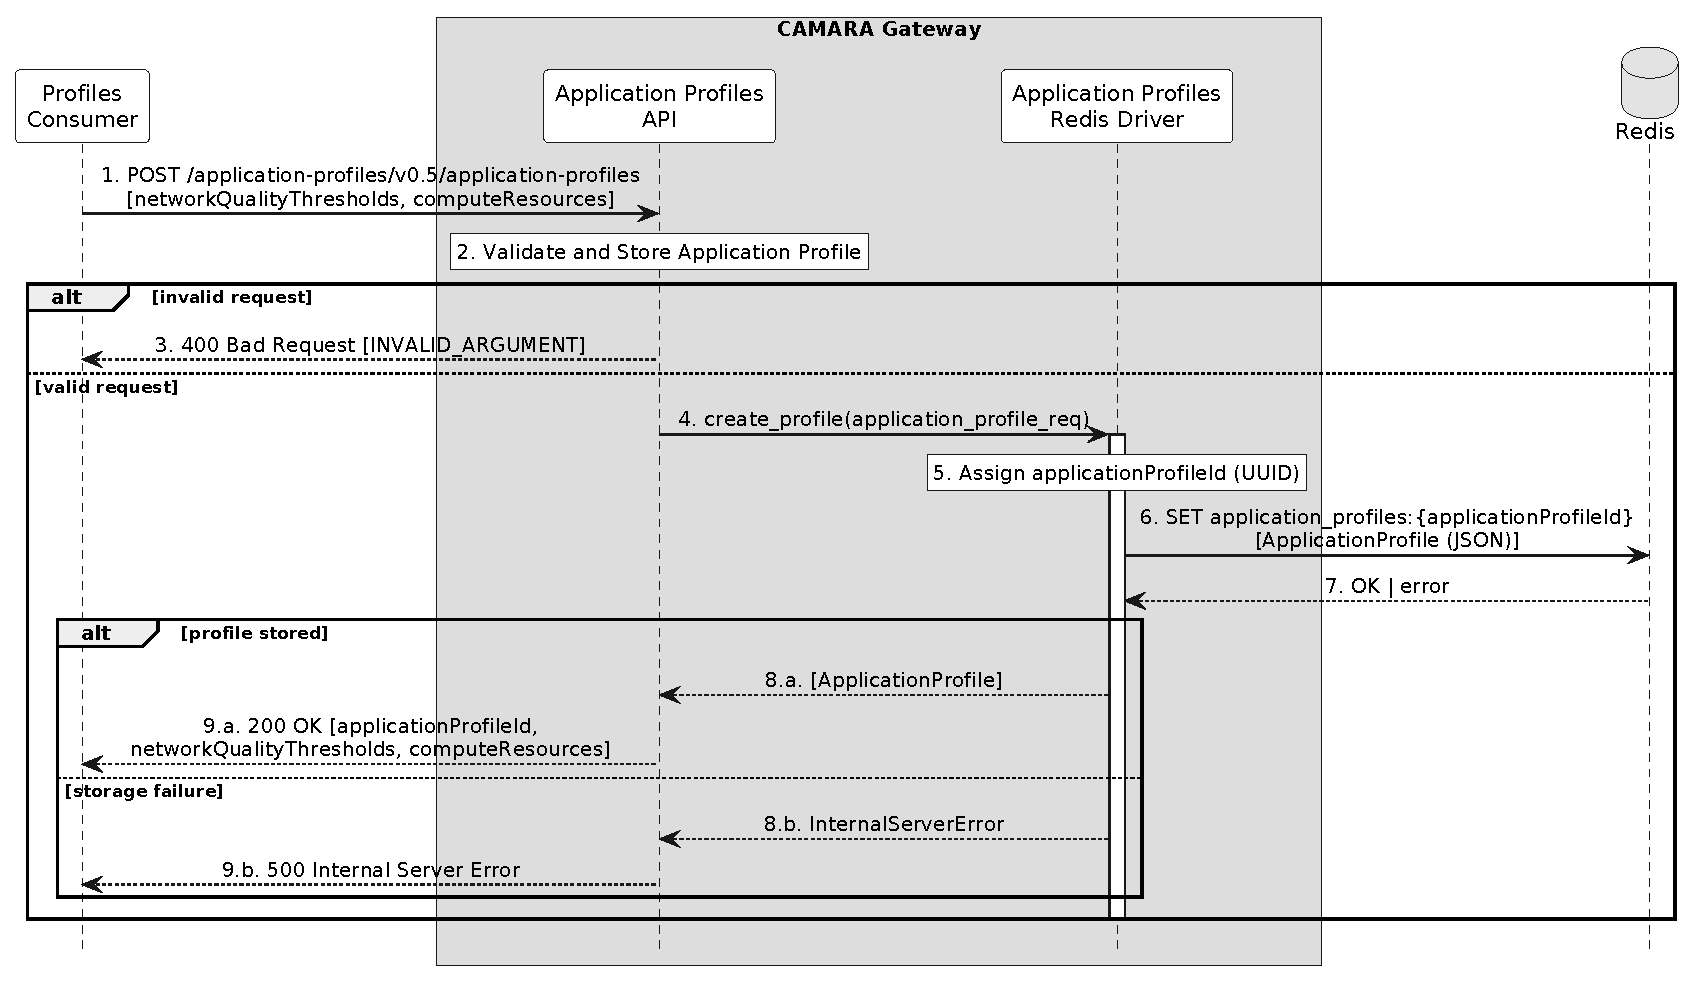
\includegraphics[width=1\linewidth]{figs/plantuml/application-profiles-sequence-create.pdf}
    \caption{Sequence Diagram for the creation of an application profile via the \textit{Application Profiles} \acs{API}}
    \label{fig:impl:exposure:camara:profiles:sequence}
\end{figure}

The interaction depicted in Figure~\ref{fig:impl:exposure:camara:profiles:sequence} is fully compliant with the \acs{NBI} realization guidelines established by \acs{GSMA}~\cite{gsmaNbiRealization} for the \textit{Application Profiles} \acs{API}, already reviewed in Section~\ref{chap:proposal:exposure:camara:profiles}. The request, declaring the network quality thresholds (and/or compute resources) required by the application, is validated and stored as an application profile. The implementation, as well as the remaining CAMARA \acsp{API} presented in this section, relies on Redis for the persistence of the created resources. This choice was first motivated by Redis being used by the already developed \acsp{API} (e.g. \acs{QoD}), which avoids introducing another persistence component. Nevertheless, it is also easily defensible from a technical stand point, as Redis closely matches the access patterns imposed by the CAMARA specifications. Every resource (e.g. an application profile, a session or a subscription) is managed exclusively through a unique identifier, which maps directly onto a key-value model. 

In this case, the profile is serialized as \acs{JSON} and stored in Redis under a key derived from a generated \acs{UUID}, i.e. the profile id, which is then returned to the client. A document-oriented database such as MongoDB would also be a viable option, but its querying capabilities would go unused, as resources are only ever accessed by identifier, making Redis the minimal option that best fits the system's needs. Finally, externalizing state to Redis keeps the exposure service stateless, allowing them to be restarted and/or horizontally scaled.

Unlike other CAMARA \acsp{API} exposed by the gateway, the \textit{Application Profiles} \acs{API} has no direct counterpart among the \acs{NEF} northbound interfaces. It is purely a management interface for application profiles, which are stored locally by the gateway without any interaction with the \acs{NEF} or the \acs{5GC}, and that are only used when referenced by other CAMARA \acsp{API}, as described next.

\subsubsection{Connectivity Insights Subscriptions}
\label{chap:impl:exposure:camara:insights}

The \textit{Connectivity Insights Subscriptions}\footnote{https://camaraproject.org/connectivity-insights-subscriptions/} \acs{API} was developed in compliance with release r3.2\footnote{https://github.com/camaraproject/ConnectivityInsights/releases/tag/r3.2} (v0.6.0), and supports the creation, retrieval, listing and deletion of analytics insights subscriptions. To provide these capabilities, the implementation interacts with the underlying \acs{NEF} to create/delete subscriptions and periodically retrieve the corresponding analytics from the configured data sources, i.e. Prometheus.

More specifically, each CAMARA subscription is realized as an \textit{AnalyticsExposure} subscription for the \texttt{WLAN\allowbreak\_PERFORMANCE} event. As discussed in Section~\ref{chap:impl:exposure:nef:AnalyticsExposure}, this event reports uplink and downlink throughput between each specified \acs{UE} and an application server. As noted earlier, this design decision departs from the \acs{GSMA} \acs{NBI} realization document~\cite{gsmaNbiRealization}, which recommended \texttt{DN\allowbreak\_PERFORMANCE}, as its associated analytics (\texttt{DnPerfInfo}) do not distinguish between uplink and downlink traffic. Table~\ref{tab:impl:exposure:camara:insights:mapping} summarizes how the fields of the CAMARA request are mapped onto the \acs{NEF} subscription.

\begin{table}[htbp]
    \centering
    \caption{\textit{Connectivity Insights Subscriptions} translation into \textit{AnalyticsExposure} subscription}
    \label{tab:impl:exposure:camara:insights:mapping}
    \begin{tabularx}{\textwidth}{@{}
        >{\RaggedRight\arraybackslash}X
        >{\RaggedRight\arraybackslash}X@{}}
        \toprule
        \textbf{\textit{Connectivity Insights Subscriptions} field} & \textbf{\textit{AnalyticsExposure} field} \\
        \midrule
        \multicolumn{2}{@{}l}{\textit{From request}} \\
        \texttt{device}                        & \texttt{tgtUe.gpsi} \\
        \texttt{applicationServer.ipv4Address} & \texttt{analyEventFilter.appServerAddrs} \\
        \texttt{subscriptionExpireTime}        & \texttt{analyRepInfo.monDur} \\
        \texttt{subscriptionMaxEvents}         & \texttt{analyRepInfo.maxReportNbr} \\
        \texttt{initialEvent}                  & \texttt{analyRepInfo.immRep} \\
        \midrule
        \multicolumn{2}{@{}l}{\textit{From configuration}} \\
        -- & \texttt{analyRepInfo.repPeriod} \\
        -- & \texttt{extraReportReq.offsetPeriod} \\
        -- & \texttt{temporalGranSize} \\
        \midrule
        \multicolumn{2}{@{}l}{\textit{Hardwired}} \\
        -- & \texttt{analyEvent} = \texttt{WLAN\_PERFORMANCE} \\
        -- & \texttt{listOfAnaSubsets} = \{\texttt{TRAFFIC\allowbreak\_INFO}, \texttt{NUMBER\allowbreak\_OF\allowbreak\_UES}\}\\
        -- & \texttt{notifMethod} = \texttt{PERIODIC} \\
        \midrule
        \multicolumn{2}{@{}l}{\textit{Replaced or not forwarded}} \\
        \texttt{sink}                          & \texttt{notifUri} = \texttt{\{gwCallback\}/\{subId\}} \\
        \texttt{applicationProfileId}          & \textit{not sent; thresholds evaluated by the gateway} \\
        \bottomrule
    \end{tabularx}
\end{table}

Each CAMARA request defines the traffic to be monitored by specifying the target device (identified by phone number or network access identifier) and the application server’s IPv4 address. It also references an application profile identifier, previously created through the \textit{Application Profiles} \acs{API}, which defines the network requirements the traffic must satisfy. Because a request accepts exactly one device, the CAMARA specification does not appear to consider monitoring multiple \acsp{UE} through a single subscription, not offering an equivalent to the \texttt{tgtUe.anyUeInd} and \texttt{tgtUe.extGroupId} parameters of the \textit{Analytics Exposure} \acs{API}. This is not specific to \textit{Connectivity Insights Subscriptions} but reflects a design decision shared across other CAMARA \acsp{API} (e.g. \acs{QoD}, Device Location) which consistently scope each request to an individual device. In this implementation, the device identifier is therefore mapped to the \acs{GPSI} of the target \acs{UE}, in the form of \texttt{msisdn-<phone number>} or \texttt{extid-<network access identifier>}. The expire time, max number of notifications and the initial event flag are also converted and forwarded on the corresponding \acs{NEF} subscription.

No other reporting parameters can be configured by the subscriber in the request. The notification method is fixed to \texttt{PERIODIC}, in accordance with the \acs{API}'s purpose of providing \textbf{periodic} connectivity insights\footnote{\url{https://raw.githubusercontent.com/camaraproject/ConnectivityInsights/r3.2/code/API_definitions/connectivity-insights-subscriptions.yaml}}. The remaining reporting parameters are therefore set at deployment time through the gateway configuration, all with a default absolute value of 5 seconds. By setting the reporting period (\texttt{repPeriod}), the analytics window (\texttt{offsetPeriod}) and the time slot duration (\texttt{temporalGranSize}) to the same value, each notification reports, in a single time slot, the uplink and downlink throughput and traffic volume observed during the interval elapsed since the previous notification. The requested analytics subsets are also explicitly set to \texttt{TRAFFIC\allowbreak\_INFO} and \texttt{NUMBER\allowbreak\_OF\allowbreak\_UES}, i.e. all metric subsets supported by \acs{NEF}Sim for the \texttt{WLAN\allowbreak\_PERFORMANCE} event.

Figure~\ref{fig:impl:exposure:camara:insights:sequence} illustrates the resulting end-to-end interaction. Starting with the creation of the analytics subscription, the request parameters are validated and the referenced application profile is retrieved from Redis, rejecting it if no such profile exists. To associate each \acs{NEF} notification with its CAMARA subscription, the subscription is assigned an \acs{UUID} that is embedded in the notification destination (\texttt{notifUri}) of the corresponding \acsp{NEF} subscription, following the translation procedure described above. The reference to the recently created \acs{NEF} subscription (\texttt{self}) is also stored in the same record for subsequent use (e.g. delete the subscription). If the \acs{NEF} rejects the request, the stored subscription is removed and the error returned to the network application (e.g. \texttt{404 Not Found} when target \acs{UE} unknown to \acs{NEF}, \texttt{500 Internal Server Error}). Notably, the thresholds of the application profile are not included in the \acs{NEF} subscription, since the \texttt{WLAN\allowbreak\_PERFORMANCE} event does not support threshold-based reporting.

\begin{figure}[htbp]
    \centering
    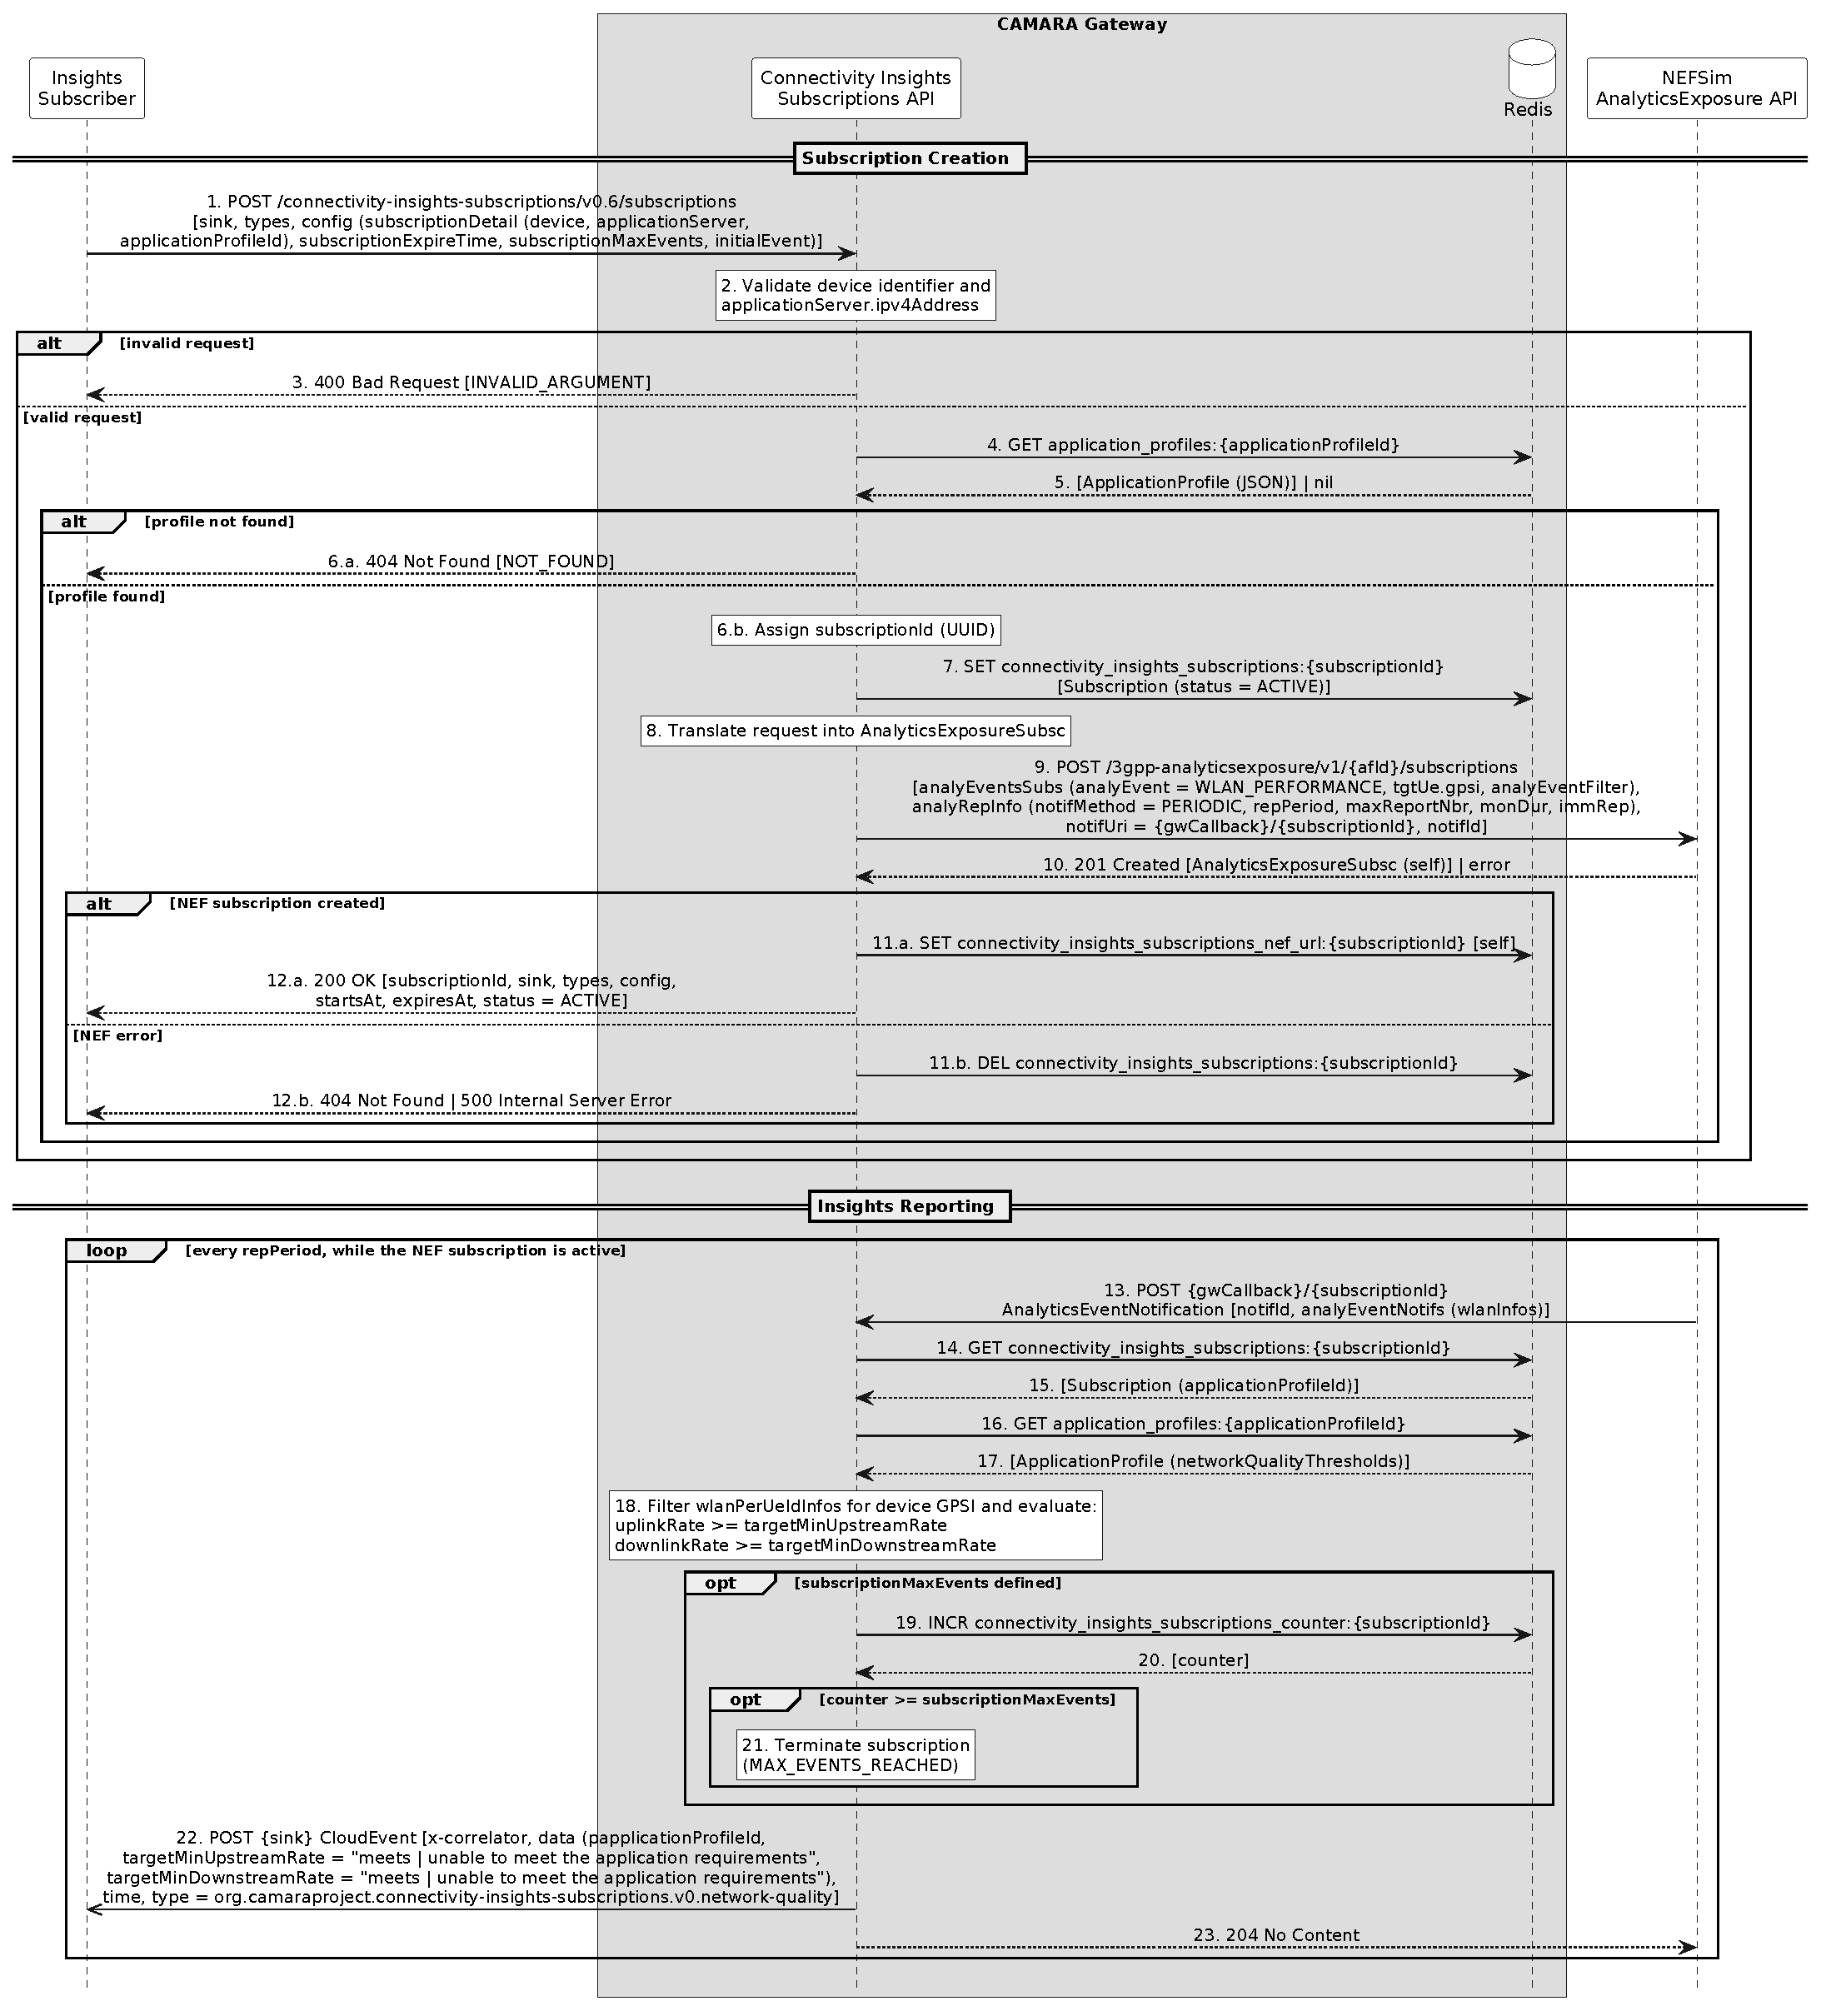
\includegraphics[width=1\linewidth]{figs/plantuml/connectivity-insights-subscription-sequence.pdf}
    \caption{Sequence Diagram for subscription creation and reporting via the \textit{Connectivity Insights Subscriptions \acs{API}}}
    \label{fig:impl:exposure:camara:insights:sequence}
\end{figure}

Instead, the \acs{NEF} periodically reports the measured uplink and downlink throughput (and volume) to the callback endpoint configured in the subscription. When a notification is received, the gateway uses the identifier provided in the callback \acs{URL} to retrieve the corresponding subscription and, subsequently the application profile. The reported uplink and downlink rates are then compared against the \texttt{targetMinUpstreamRate} and \texttt{targetMinDownstreamRate} thresholds of the profile. Each threshold is then classified as either \textit{meets the application requirements} or \textit{unable to meet the application requirements}. The resulting network quality insight, i.e. the threshold compliance status, is delivered to the original CAMARA subscriber as a background task (if max reports haven't been reached), specified in \textit{sink}. This is also characteristic of CAMARA. The notification gets relayed and may undergo some additional processing that enriches the results. The remaining network quality thresholds, i.e. packet delay budget, packet error loss rate and jitter, are not evaluated, as the testbed's passive monitoring component does not cover such metrics (Section~\ref{chap:impl:observability}).

Subscription termination reuses the subscription logic shared by other CAMARA subscription \acsp{API} of the gateway, such as Geofencing Subscriptions. A subscription is terminated when the network application deletes it, the maximum number of events is reached, its expiration time elapses, or the \acs{NEF} reports its termination. In all cases, the subscription is marked as inactive, the corresponding \acs{NEF} subscription is deleted (in the background, if it is not already), and a \texttt{subscription-ended} notification indicating the termination reason is sent to the sink.

Combined, the \textit{Application Profiles} and \textit{Connectivity Insights Subscriptions} \acsp{API} turn the raw analytics of the \textit{AnalyticsExposure} \acs{API} into application-level information. This simplifies the integration of network analytics, shielding application developers from the diversity of analytics events and payloads exposed by the underlying \acs{API}. Instead of requiring developers to interpret these analytics, manage \acs{3GPP} subscriptions, and evaluate reported metrics against application-specific thresholds, a network application declares its requirements in a profile, subscribes with the corresponding identifier, and receives a per-threshold verdict on whether the network meets them. This logic, otherwise repeated by every application relying on the \acs{NEF} directly, is thus concentrated in the exposure layer of the testbed and abstracted from the user.
